\documentclass{report}
\usepackage{float}
\usepackage{tabularx}
\usepackage{amsmath,amssymb,amsfonts}
\usepackage{algorithmic}
\usepackage{graphicx,color}

\begin{document}
\section*{ This is one single example of simulation with all details plot describing the models }
\begin{itemize}
    \item \textbf{p=3000} (number of covariates)
    \item \textbf{n=200} (observations)
    \item  \textbf{s=5} (number of non-zero coefficients among 3000 coefficients) is the size of the active set.
\end{itemize}
\subsection*{True Lasso model}

\begin{figure}[H]
	\centering
		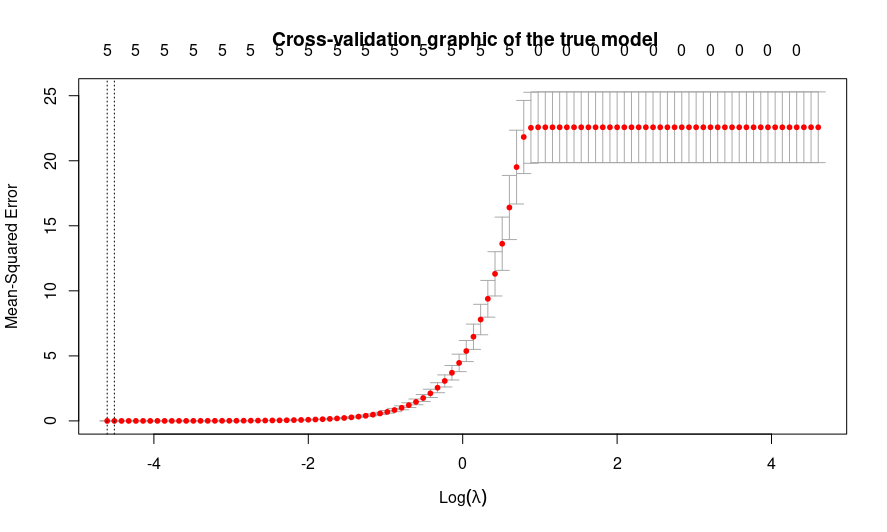
\includegraphics[scale=0.5]{pictures/cvtl.png}
	\caption{Cross validation of the true Lasso model}
	\label{t1}
\end{figure}

\begin{figure}[H]
	\centering
		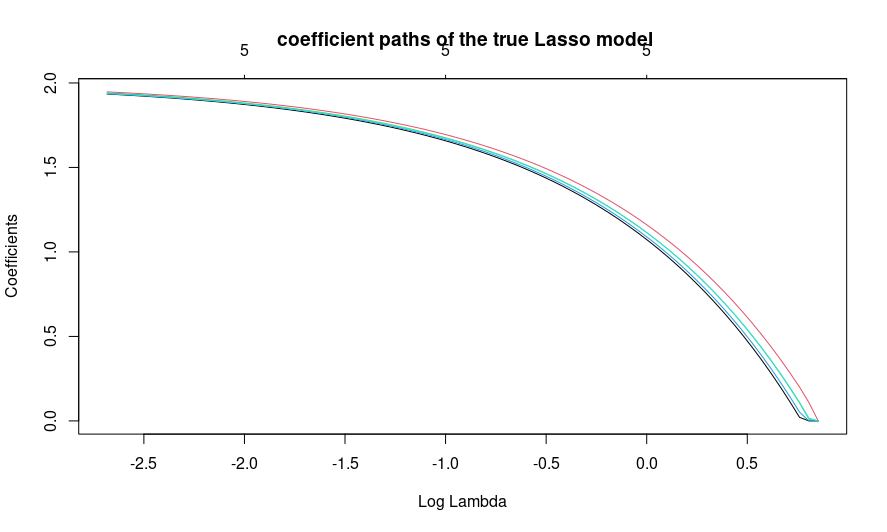
\includegraphics[scale=0.4]{pictures/ptl.png}
	\caption{Coefficient paths of the true Lasso model}
	\label{t2}
\end{figure}

\begin{figure}[H]
	\centering
		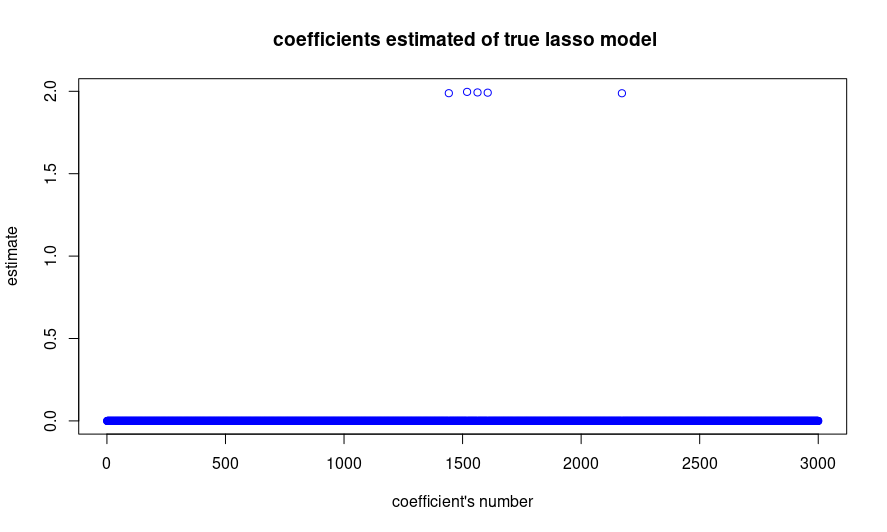
\includegraphics[scale=0.4]{pictures/cetl.png}
	\caption{Coefficients estimated of the true Lasso model}
	\label{t3}
\end{figure}

\subsection*{Naive Lasso Model}
\begin{figure}[H]
	\centering
		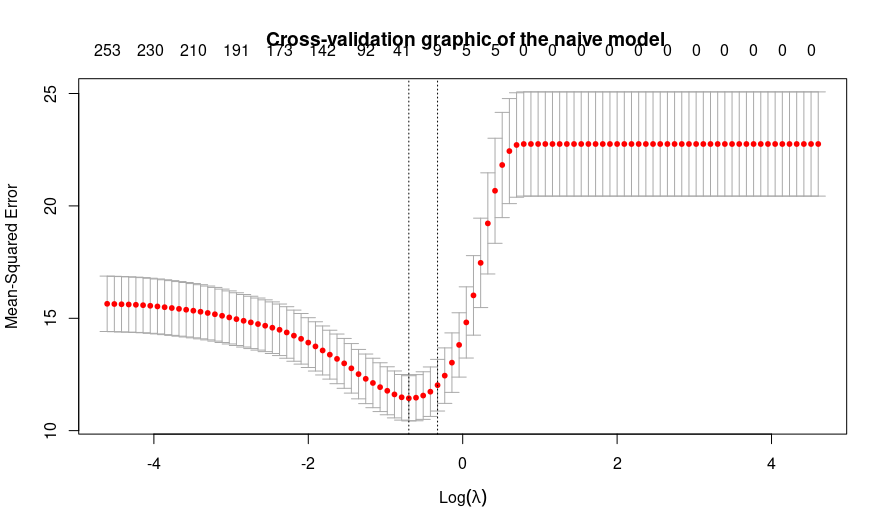
\includegraphics[scale=0.5]{pictures/cvnl.png}
	\caption{Cross validation of the Naive Lasso model}
	\label{t4}
\end{figure}

\begin{figure}[H]
	\centering
		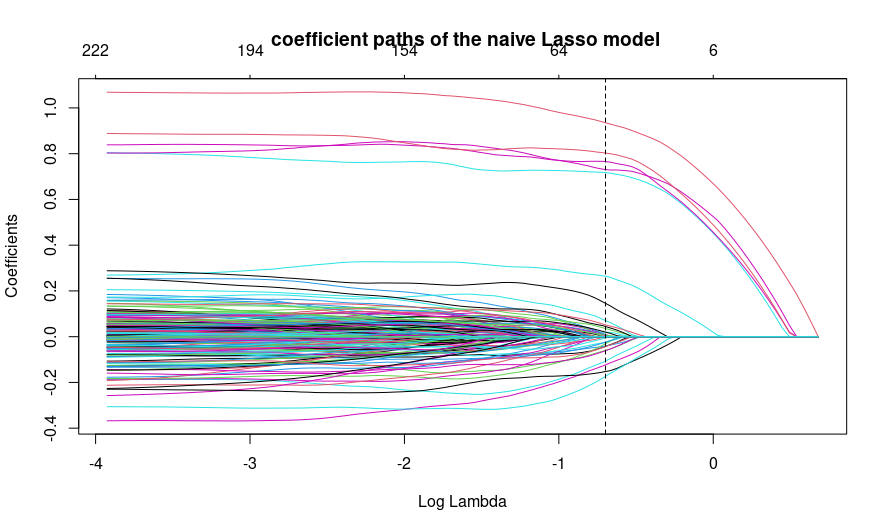
\includegraphics[scale=0.5]{pictures/pnl.png}
	\caption{Coefficient paths of the Naive Lasso model}
	\label{t5}
\end{figure}

\begin{figure}[H]
	\centering
		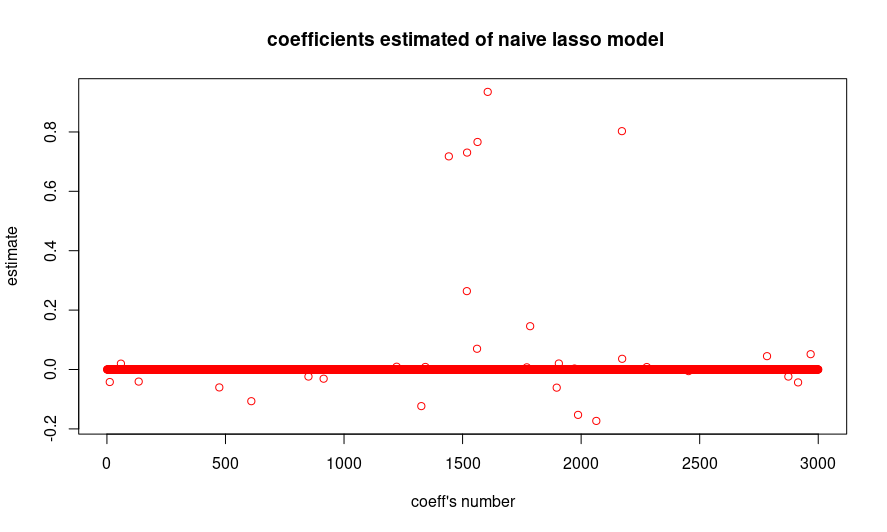
\includegraphics[scale=0.5]{pictures/cenl.png}
	\caption{Coefficients estimated of the Naive Lasso model}
	\label{t6}
\end{figure}

\subsection*{Non Convex Lasso (NCL) }
\begin{figure}[H]
	\centering
		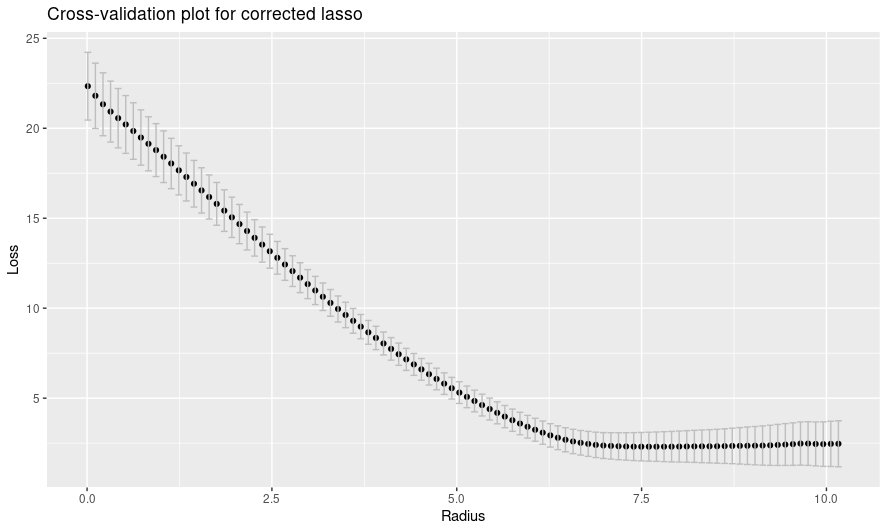
\includegraphics[scale=0.5]{pictures/cvcl.png}
	\caption{Cross validation of the NCL model}
	\label{t7}
\end{figure}

\begin{figure}[H]
	\centering
		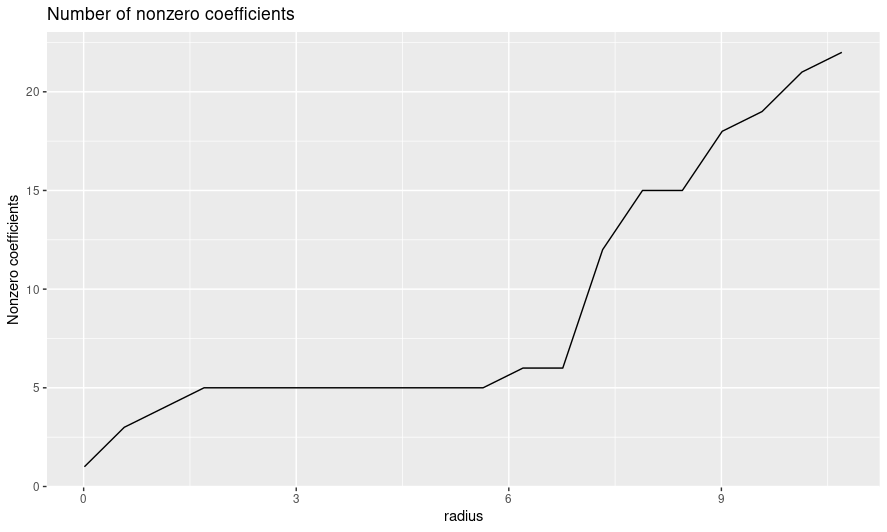
\includegraphics[scale=0.5]{pictures/nnccl.png}
	\caption{NCL: Evolution of Nonzero coefficients with respect to  Radius (R)}
	\label{t8}
\end{figure}

\begin{figure}[H]
	\centering
		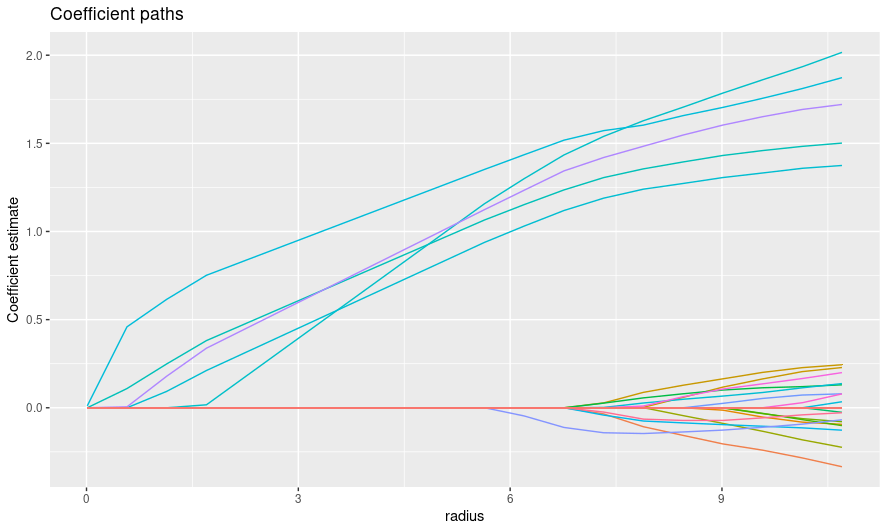
\includegraphics[scale=0.5]{pictures/pcl.png}
	\caption{Coefficient paths of the NCL model}
	\label{t9}
\end{figure}

\begin{figure}[H]
	\centering
		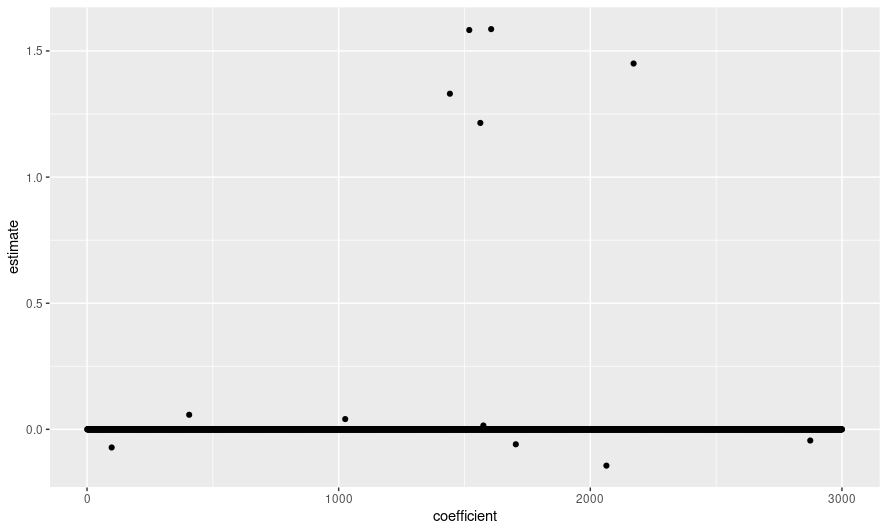
\includegraphics[scale=0.5]{pictures/cecl.png}
	\caption{Coefficients estimated of the NCL model}
	\label{t10}
\end{figure}

\subsection*{Convex Conditional Lasso ( CoCoLasso)}
\begin{figure}[H]
	\centering
		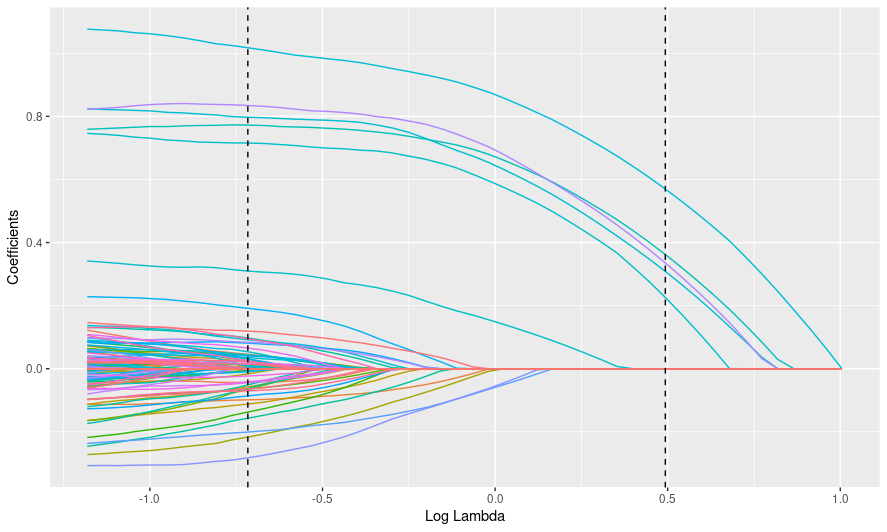
\includegraphics[scale=0.5]{pictures/pcocol.png}
	\caption{Coefficients paths of the CoCoLasso model}
	\label{t11}
\end{figure}

\begin{figure}[H]
	\centering
		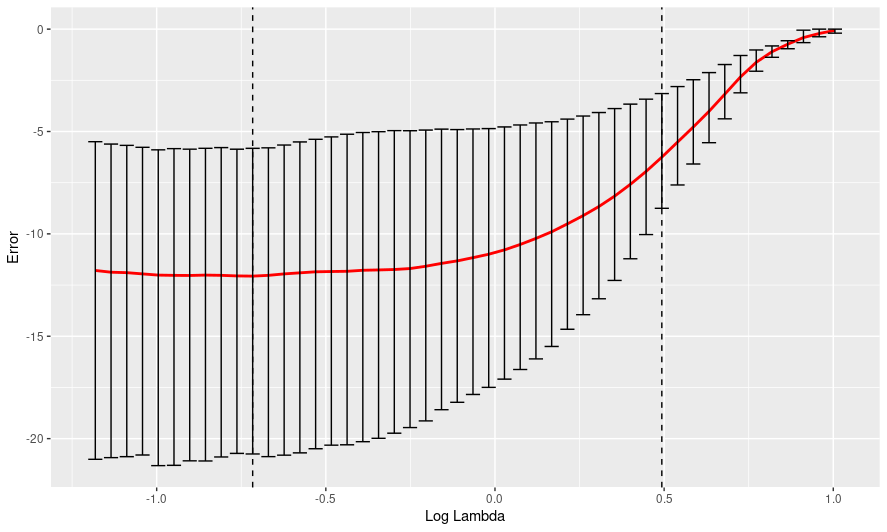
\includegraphics[scale=0.5]{pictures/msecocol.png}
	\caption{Cross-Validation of the CoCoLasso model}
	\label{t12}
\end{figure}

\subsection{Matrix Uncertainty selector (MUS) }
\begin{figure}[H]
	\centering
		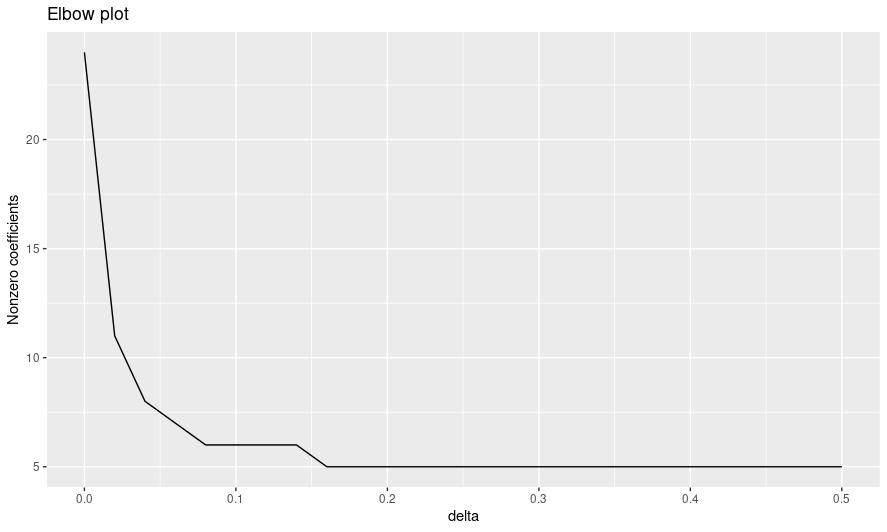
\includegraphics[scale=0.5]{pictures/nzcmus.png}
	\caption{Graphic (MUS) :path of Nonzero coefficients along the grid of "$\delta$"  ( to apply the Elbow rule)}
	\label{t13}
\end{figure}

\begin{figure}[H]
	\centering
		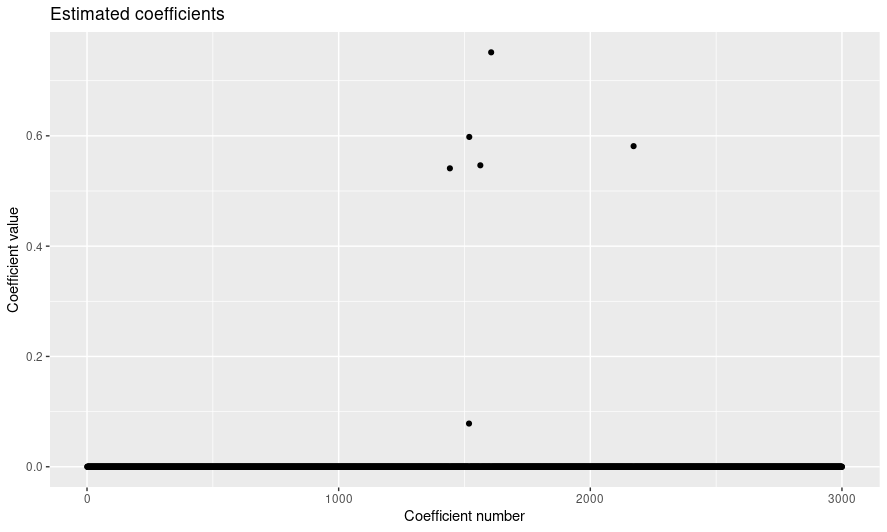
\includegraphics[scale=0.5]{pictures/cemus.png}
	\caption{Graphic(MUS) : Coefficients estimated of the MUS model }
	\label{t14}
\end{figure}
\end{document}